 %\documentclass[handout]{beamer}
%\documentclass{beamer}
\documentclass[aspectratio=169]{beamer}



\usepackage [latin1] {inputenc}		% LaTeX, comprends les accents !
\usepackage [T1] {fontenc}      		% Police contenant les caractères français
\usepackage {geometry}         		% Définir les marges
\usepackage [english] {babel}  	
%\usepackage[backend=biber]{biblatex}
%\bibliography{bib.bib}
\setbeamertemplate{bibliography item}[text]
\usepackage{color}
\usepackage{wasysym}
\usepackage{xcolor}
\usepackage{cancel}
\usepackage{fancybox}
\usepackage{changepage}
\usepackage{tcolorbox}


\usepackage[export]{adjustbox}
\usepackage{tabulary}
\newcolumntype{K}[1]{>{\centering\arraybackslash}p{#1}}

\usepackage{booktabs}
\usepackage{multirow}
\usepackage{fixltx2e}

\usepackage{fancyvrb}
\usepackage {graphicx}
\usepackage{url}
\usepackage {amsmath}
\usepackage {array}
\usepackage {tikz}
\usepackage{pgfkeys}
\usetikzlibrary{shapes,arrows}
\usepackage {subfigure}												% Pour les subfigures
\usepackage{enumitem}
\usepackage{bm}

\usepackage{algorithm}
\usepackage{algpseudocode}
\usepackage{caption} % For caption*
\usepackage{fontawesome}


%\usepackage{eso-pic}    % Pour ajouter des éléments en arrière-plan

%\setlist[itemize,1]{label=$\times$}%
%\setlist[itemize,2]{label=$\checkmark$}
\setlist[itemize,1]{label=$\diamond$}
\setlist[itemize,2]{label=$-$}

\usepackage{listings} 
%\usepackage{color}

\definecolor{mygreen}{rgb}{0,0.6,0}
\definecolor{mygray}{rgb}{0.5,0.5,0.5}
\definecolor{mymauve}{rgb}{0.58,0,0.82}

\lstset{ %
backgroundcolor=\color{white},   % choose the background color; you must add \usepackage{color} or \usepackage{xcolor}; should come as last argument
basicstyle=\footnotesize,        % the size of the fonts that are used for the code
breakatwhitespace=false,         % sets if automatic breaks should only happen at whitespace
breaklines=true,                 % sets automatic line breaking
captionpos=b,                    % sets the caption-position to bottom
commentstyle=\color{mygreen},    % comment style
deletekeywords={...},            % if you want to delete keywords from the given language
escapeinside={\%*}{*)},          % if you want to add LaTeX within your code
extendedchars=true,              % lets you use non-ASCII characters; for 8-bits encodings only, does not work with UTF-8
frame=single,	                   % adds a frame around the code
keepspaces=true,                 % keeps spaces in text, useful for keeping indentation of code (possibly needs columns=flexible)
keywordstyle=\color{blue},       % keyword style
language=Octave,                 % the language of the code
morekeywords={*,...},           % if you want to add more keywords to the set
numbers=left,                    % where to put the line-numbers; possible values are (none, left, right)
numbersep=5pt,                   % how far the line-numbers are from the code
numberstyle=\tiny\color{mygray}, % the style that is used for the line-numbers
rulecolor=\color{black},         % if not set, the frame-color may be changed on line-breaks within not-black text (e.g. comments (green here))
showspaces=false,                % show spaces everywhere adding particular underscores; it overrides 'showstringspaces'
showstringspaces=false,          % underline spaces within strings only
showtabs=false,                  % show tabs within strings adding particular underscores
stepnumber=1,                    % the step between two line-numbers. If it's 1, each line will be numbered
stringstyle=\color{mymauve},     % string literal style
tabsize=2,	                   % sets default tabsize to 2 spaces
title=\lstname                   % show the filename of files included with \lstinputlisting; also try caption instead of title
}

%\setbeamersize{text margin left=1.5cm} 
\definecolor{HardTitle}{RGB}{50,50,160}
\definecolor{LightT}{RGB}{0,0,255}
\definecolor{cadmiumgreen}{rgb}{0.0, 0.42, 0.24}
\beamerboxesdeclarecolorscheme{clair}{LightT}{white}
\usetheme[]{default}

\usecolortheme{default}
%\setbeamercolor{frametitle}{fg=HardTitle, bg=white}
\useinnertheme{default}
\useoutertheme{default}
\setbeamertemplate{footline}{\begin{flushright} \insertframenumber \hspace*{0.5cm} \end{flushright} }
\setbeamertemplate{navigation symbols}{}

\setbeamertemplate{itemize item}{\textbullet}
\setbeamertemplate{itemize subitem}{\textbullet}


%%%%%%%%%%%%%%%%%%% PLOTS
\usepackage{pgfplots}
%\usetikzlibrary{external}
%\tikzexternalize[prefix=Numerical_results/]
\pgfplotsset{compat=1.13}


\tikzstyle{loosely dashed}=          [dash pattern=on 3pt off 6pt]
\pgfplotsset{plotOptions/.style={%
%		y post scale=0.8,
%		ymin=0,ymax=100,
%		ymin=0,
%		xmin=0,xmax=100,
%xlabel={Iteration counter $k$},
%ylabel={$f(x_k)-f(x_\star)$},
%label style={font=},
%legend style={font=},
%		legend pos=north west,
%		legend cell align=left,
%yticklabels=\empty,
%xticklabels=\empty,
%tick label style={font=},
%		no markers,
solid,
very thick
}}
\pgfplotsset{plotOptions2/.style={%
		%		y post scale=0.8,
		%		ymin=0,ymax=100,
		%		ymin=0,
		%		xmin=0,xmax=100,
		xlabel={Lipschitz constant $L$},
		ylabel={Contraction rate $\rho^2$},
		label style={font=\tiny},
		legend style={font=\tiny},
		%		legend pos=north west,
		%		legend cell align=left,
		%yticklabels={0,1},
		%xticklabels={0,1},
		tick label style={font=\tiny},
		%		no markers,
		solid,
		very thick
	}}
\pgfplotsset{plotOptions3/.style={%
		%		y post scale=0.8,
		%		ymin=0,ymax=100,
		%		ymin=0,
		%		xmin=0,xmax=100,
		xlabel={Iteration counter $k$},
		ylabel={$f(x_k)-f(x_\star)$},
		label style={font=\tiny},
		legend style={font=\tiny},
		%		legend pos=north west,
		%		legend cell align=left,
		yticklabels=\empty,
		xticklabels=\empty,
		tick label style={font=\tiny},
		%		no markers,
		solid,
		very thick
	}}
\pgfplotsset{plotOptions4/.style={%
		width=\linewidth,
		%		y post scale=0.8,
				ymax=100,ymin=.0000001,
		%		ymin=0,
				xmin=0,xmax=50,
		xlabel={Iteration $N$},
		ylabel={$\frac{f(x_N)-f_\star}{\|x_0-x_\star\|^2}$},
		%		ylabel={Evaluations to convergence},
		label style={font=\small},
		legend style={font=\small},
		%		legend pos=north west,
		%		legend cell align=left,
		ytick={10,.001,.0000001},
		xtick={0,10,20,30,40,50},
		tick label style={font=\small},
		%		no markers,
		solid,
		very thick
	}}
	\pgfplotsset{plotOptions5/.style={%
			width=\linewidth,
			%		y post scale=0.8,
			ymax=10,ymin=.00001,
			%		ymin=0,
			xmin=0,xmax=50,
			%		ymin=0,ymax=100,
			%		ymin=0,
			%		xmin=0,xmax=100,
			xlabel={Iteration $N$},
			ylabel={$\frac{f(x_N)-f_\star}{f(x_0)-f_\star}$},
			%		ylabel={Evaluations to convergence},
			label style={font=\small},
			legend style={font=\small},
			%		legend pos=north west,
			%		legend cell align=left,
			%xtick={1,10,100},
			tick label style={font=\small},
			ytick={1,.01,.0001},
			xtick={0,10,20,30,40,50},
			%		no markers,
			solid,
			very thick
		}}	
	
	\pgfplotsset{plotOptionsNeutral/.style={%
			%		y post scale=0.8,
			%		ymin=0,ymax=100,
			%		ymin=0,
			%		xmin=0,xmax=100,
			xlabel={``Time''},
			ylabel={``Error''},
			label style={font=\small},
			%		legend style={font=\tiny},
			%		legend pos=north west,
			%		legend cell align=left,
			yticklabels={},
			xticklabels={},
			%		tick label style={font=\tiny},
			%		xtick label style={no markers},
			%		ytick label style={no markers},
			solid,
			very thick
	}}
%%%%%%%%%%%%%%%%%%%%%%%%%%%
%%%%%%%%%%%%%%%%%%%%%%%%%%% COLORS


\definecolor{silver}{cmyk}{0,0,0,0.3}
\definecolor{yellow}{cmyk}{0,.5,.3,0}
\definecolor{orange}{cmyk}{0,0.5,1,0}
\definecolor{red}{cmyk}{0,1,1,0}
\definecolor{reddishyellow}{cmyk}{0.5,0.2,0,0}
\definecolor{black}{cmyk}{0,0,0.0,1.0}
\definecolor{darkYellow}{cmyk}{0.8,0,0.0,0.5}
\definecolor{darkSilver}{cmyk}{0,0,0,0.1}

\definecolor{lightyellow}{cmyk}{0.0,0,0,0.0}
\definecolor{lighteryellow}{cmyk}{0,0,0.0,0.0}
\definecolor{lighteryellow}{cmyk}{0,0,0.0,0.0}
\definecolor{lightestyellow}{cmyk}{0.0,0,0.0,0.0}

\definecolor{colorP1}{RGB}{55,126,184}  % blue
\definecolor{colorP2}{RGB}{228,26,28}  % red
\definecolor{colorP3}{RGB}{152,78,163} % purple
\definecolor{colorP4}{RGB}{77,175,74}  % green
\definecolor{colorP5}{rgb}{0.6, 0.4, 0.08} % golden yellow
%%%%%%%%%%%%%%%%%%%%%%%%%%%
\makeatletter
\pgfplotsset{
every axis x label/.append style={
alias=current axis xlabel,
},
legend pos/outer south/.style={
/pgfplots/legend style={
	at={%
		(%
		\@ifundefined{pgf@sh@ns@current axis xlabel}%
		{xticklabel cs:0.5}%
		{current axis xlabel.south}%
		)%
	},
	anchor=north
},
},
}
\makeatother
%%%%%%%%%%%%%%%%%%%%%%%%%%%
\definecolor{mycolorOne}{RGB}{255,0,0}
\definecolor{mycolorTwo}{RGB}{0,157,255}
\definecolor{mycolorThree}{RGB}{204,201,0}
\definecolor{mycolorFour}{RGB}{237,127,16}

\definecolor{darkcandyapplered}{rgb}{0.64, 0.0, 0.0}
\definecolor{darkspringgreen}{rgb}{0.09, 0.45, 0.27}
\definecolor{deepcarrotorange}{rgb}{0.91, 0.41, 0.17}

\newcommand{\norm}[1]{{\left\lVert#1\right\rVert}}
\newcommand{\normpsq}[1]{{\left\lVert#1\right\rVert}^2}
\newcommand{\normsq}[1]{{\left\lVert#1\right\rVert}^2}
\newcommand{\normdsq}[1]{{\left\lVert#1\right\rVert}^2}
\newcommand{\inner}[2]{{\left< #1, #2\right>}}
\newcommand{\argmin}[1]{\underset{#1}{\text{argmin }}}
\newcommand{\argmax}[1]{\underset{#1}{\text{argmax }}}
\newcommand{\maxim}[1]{\underset{#1}{\text{max }}}
\newcommand{\suprem}[1]{\underset{#1}{\text{sup }}}
\newcommand{\minim}[1]{\underset{#1}{\text{min }}}
\newcommand{\goto}[1]{\overset{\mu\rightarrow 0}{\rightarrow}#1}
\newcommand{\prox}[2]{\underset{#1}{\mathrm{prox}\left(#2\right)}}
\newcommand{\real}{\mathbb{R}}
\newcommand{\emphcolor}[1]{\emph{\color{red}#1}}
\newcommand{\cond}{\tfrac{\mu}{L}}
\newcommand{\bc}[1]{{\color{blue}#1}}
\newcommand{\rc}[1]{{\color{red}#1}}
\newcommand{\cc}[1]{{\color{cyan}#1}}
\newcommand{\co}[1]{{\color{orange}#1}}
\newcommand{\defeq}{\overset{\text{(def)}}{=}}

\newcommand{\hilbert}{\mathcal{H}}
\DeclareMathOperator{\dom}{dom}
\DeclareMathOperator{\val}{val}
\DeclareMathOperator{\epi}{epi}
\DeclareMathOperator{\trace}{Tr}
\DeclareMathOperator{\tr}{\trace}
\DeclareMathOperator{\linspan}{span}
\DeclareMathOperator{\rank}{rank}
\DeclareMathOperator{\FmuL}{\mathcal{F}_{\mu,L}}
\usepackage{pifont} 
\author{Adrien Taylor}
\title{}
\institute [] {}\date{\today}

\renewcommand{\leq}{\leqslant}
\renewcommand{\geq}{\geqslant}
\renewcommand{\succeq}{\succcurlyeq}
\renewcommand{\preceq}{\preccurlyeq}


%\setbeamersize{text margin left=5pt,text margin right=25pt}
\setbeamerfont{footnote}{size=\tiny}
\setbeamersize{text margin left=6mm,text margin right=6mm} 
\usepackage{changepage}

\newcommand{\picsizeo}{.13}
\newcommand{\picsizeth}{.09}
\newcommand{\picsizet}{.10}
\definecolor{someBlue}{rgb}{0,0,2}
\definecolor{someOrange}{rgb}{0.9290, 0.6940, 0.1250}
\definecolor{darkgreen}{rgb}{0.0, 0.5, 0.0}
\newcommand{\titleB}[1]{{}|\! #1}
\newcommand{\frtitle}[1]{\frametitle{\titleB{#1}}}
\begin{document}


\begin{frame}
\thispagestyle{empty}
\setcounter{framenumber}{0}
\begin{center}
\textcolor{HardTitle}{\Large{}Performance Estimation Problems (PEPs)\\[.5cm]}
 \textcolor{HardTitle}{Systematic, principled, and computer-aided approaches\\to the analysis and design of first-order optimization algorithms}
\end{center}
\normalsize
\vspace{.7cm}
\begin{center}
\small {{Aymeric Dieuleveut, \underline{Adrien Taylor}}} \\[.5cm]

\includegraphics[width=.2\linewidth]{Logos/X.png}\hspace{2cm} 
\includegraphics[width=.2\linewidth]{Logos/inr_logo_rouge_pms.eps}\hspace{2cm} 
\includegraphics[width=.2\linewidth]{Logos/logo_ens_psl_couleur.png}\\[1cm]

\scriptsize SMAI-MODE tutorial -- March 2026

\end{center}
\end{frame}




\begin{frame}
	\Large
	\tableofcontents
\end{frame}
\section{Forewords and problem statement}
\begin{frame}
	\Large
	\tableofcontents [currentsection, hideothersubsections]
\end{frame}

\begin{frame}
\frtitle{Creating new algorithms}\small\vspace{.3cm}
\uncover<1->{A ``generic'' first-order method \begin{equation}\label{eq:ogm_start}\tag{FOM}
		\begin{aligned}
		w_1 &= w_0 - \bc{\alpha_{1,0}}  \nabla f (w_0)\\
		w_2 &= w_1 - \bc{\alpha_{2,0}}  \nabla f (w_0) - \bc{\alpha_{2,1}} \nabla f (w_1)\\
		w_3 &= w_2 - \bc{\alpha_{3,0}}  \nabla f (w_0) - \bc{\alpha_{3,1}} \nabla f (w_1) - \bc{\alpha_{3,2}}  \nabla f (w_2)\\
		&\vdots\\
		w_N &= w_{N-1} - \sum_{i=0}^{N-1} \bc{\alpha_{N,i}} \nabla f (w_i),
		\end{aligned}
		\end{equation}
		for some coefficients $\{\bc{\alpha_{i,j}}\}$. Generic \textbf{non-adaptive} first-order method.}\\[.4cm]

\uncover<2->{How to choose $\{\bc{\alpha_{i,j}}\}$? 
\begin{itemize}
	\item<3-> pick a performance criterion, for instance $\frac{\|w_N-w_\star\|^2}{\|w_0-w_\star\|^2}$,
	\item<4-> solve the minimax (minimize worst-case):
$\underset{\{\bc{\alpha_{i,j}}\}_{i,j}}{\min}\,\,\underset{f\in\mathcal{F},\{w_i\}}{\max} \frac{\|w_N-w_\star\|^2}{\|w_0-w_\star\|^2}$.
\end{itemize}}
\end{frame}

\begin{frame}\frtitle{Traditional design}\small\vspace{.3cm}

	Algorithm design (with guarantees):	
	\begin{itemize}
		\item<2-> unconstrained quadratic programming:
			\begin{itemize}
				\item[] first-order methods $\Leftrightarrow$ polynomials $\rightarrow$ optimal algorithms via optimal polynomials.\footnote<2->{Golub and Varga (1961). ``Chebyshev semi-iterative methods, successive
overrelaxation iterative methods, and second order Richardson iterative methods.'' Numerische Mathematik.}\textsuperscript{,}\footnote<2->{Polyak (1987). ``Introduction to optimization.'' Optimization Software.}\textsuperscript{,}\footnote<2->{Nemirovski (1995). ``Information-based complexity of convex programming.'' (Lecture notes)}
			\end{itemize}
		\item<3-> Beyond quadratics: traditionally more ``hand-crafted''
		\begin{itemize}
			\item Analogy with conjugate gradients.\footnote<3->{Nemirovski (1982). ``Orth-method for smooth convex optimization.'' (in Russian) Engineering Cybernetics.}\textsuperscript{,}\footnote<3->{Narkiss and Zibulevsky (2005). ``Sequential subspace optimization method for large-scale unconstrained problems.''}
			\item Lyapunov function-type analyses.\footnote<3->{Nesterov (1983). ``A method for solving the convex programming problem with convergence rate $O(1/k^2)$.'' Dokl. akad. nauk. Sssr 269.}\textsuperscript{,}\footnote<3->{Beck and Teboulle (2009). ``A fast iterative shrinkage-thresholding algorithm for linear inverse problems.'' SIAM journal on imaging sciences 2(1).
}
		\end{itemize}
	\end{itemize}
\end{frame}



\begin{frame}\frtitle{Design problem}\small\vspace{.3cm}

How to solve the design problem (or proxy of it)?
	\[ {\color{red}\min_{\{\bc{\alpha_{i,j}}\}}\max_{f\in\mathcal{F}} \frac{\|w_N-w_\star\|^2}{\|w_0-w_\star\|^2}}?\uncover<2->{\quad \min_{\{\bc{\alpha_{i,j}}\}}\max_{f\in\mathcal{F}} \frac{f(w_N)-f(w_\star)}{f(w_0)-f(w_\star)}?}\uncover<3->{\quad \min_{\{\bc{\alpha_{i,j}}\}}\max_{f\in\mathcal{F}} \frac{\|\nabla f(w_N)\|^2}{\|\nabla f(w_0)\|^2}?}\]
	\begin{itemize}
		\item<4-> Convex relaxations,
		\item<5-> analogies (e.g., with conjugate gradient methods)
		\[ w_{k+1}\in\ \underset{x\in \mathbb{R}^d}{\mathrm{argmin}} \left\{f(w):\; w\in w_0+\mathrm{span}\{\nabla f(w_0),\hdots,\nabla f(w_{k})\}\right\},\]
		\item<6-> brutal approaches.
	\end{itemize}
	
\end{frame}
\frame{\frtitle{Primal problem ($N=1$)}\scriptsize
			\vspace{.3cm}\uncover<2->{Recall primal problem, with step-size optimization \begin{equation*}
				\begin{aligned}
				\minim{\bc{\alpha_{1,0}}}\,\,\maxim{G,\, F} \quad & {G_{1,1}+\bc{\alpha_{1,0}^2} G_{2,2}-2\bc{\alpha_{1,0}}G_{1,2}}\\
				\text{subject to } \quad & F + \tfrac{L\mu}{2(L-\mu)} G_{1,1}+\tfrac{1}{2(L-\mu)}G_{2,2}-\tfrac{L}{L-\mu}G_{1,2}\leqslant 0\\
				&-F + \tfrac{L\mu}{2(L-\mu)} G_{1,1}+\tfrac{1}{2(L-\mu)}G_{2,2}-\tfrac{\mu}{L-\mu}G_{1,2}\leqslant 0\\
				&G_{1,1}= 1\\
				&G\succcurlyeq 0.
					\end{aligned}
				\end{equation*}}
			
			\uncover<3->{``Simple'' minimization problem by dualizing inner maximization.}\\[.3cm]
			
			\uncover<4->{Dualize inner maximization $\rightarrow$ $\min \min$.}
			}
	
		\frame{\frtitle{Optimizing the step-sizes  ($N=1$)}\vspace{.3cm}\scriptsize
		
		\uncover<2->{ For $N=1$, {\color{red}optimizing over step-size $\bc{\alpha_{1,0}}$} remains convex!}\\[.3cm]
		
		\uncover<3->{Indeed:
				{\begin{align*}
					\minim{\co{\tau},\co{\lambda}\geqslant 0\uncover<4->{,{\bc{\alpha_{1,0}}}}} & \,\co{\tau}\\
					\text{subject to }& \begin{bmatrix}
					\co{\tau}-1+\frac{ \co{\lambda} L\mu}{L-\mu }  & \bc{\alpha_{1,0}}-\frac{\co{\lambda} (\mu +L)}{2 (L-\mu )} \\
					\bc{\alpha_{1,0}}-\frac{\co{\lambda} (\mu +L)}{2 (L-\mu )} & \frac{\co{\lambda}}{L-\mu }-\bc{\alpha_{1,0}^2} \\
					\end{bmatrix}\succcurlyeq 0.\\
					\end{align*}
				}}
		
		\uncover<5->{Optimize ${\bc{\alpha_{1,0}}}$ ``for free'' (linear SDP via Schur complement):
				{\begin{align*}
					\minim{\co{\tau},\co{\lambda}\geqslant 0\uncover<4->{,{\bc{\alpha_{1,0}}}}} & \,\co{\tau}\\
					\text{subject to }& \begin{bmatrix}
					\co{\tau}-1+\frac{\co{\lambda} L\mu}{L-\mu }  &
					-\frac{\co{\lambda} (\mu +L)}{2 (L-\mu )} & 1\\
					-\frac{\co{\lambda} (\mu +L)}{2 (L-\mu )} & \frac{\co{\lambda}}{L-\mu } & -\bc{\alpha_{1,0}}\\
					1 & -\bc{\alpha_{1,0}} & 1 \\
					\end{bmatrix}\succcurlyeq 0.\\
					\end{align*}}
				}}



			
\begin{frame}\frtitle{Optimizing the step-sizes  ($N=2$)}\vspace{.3cm}\scriptsize
			
			When $N=2$, the problem becomes
					\begin{equation*}
					\begin{aligned}
						\min_{\substack{\co{\tau},\co{\lambda_1},\hdots,\co{\lambda_6}\geqslant 0\\ \{\bc{\alpha_{i,j}}\}}}\,& \tau\\
						\text{subject to }& \uncover<3->{{\begin{bmatrix} S_{1,1} & S_{1,2} &  S_{1,3} \\
							  S_{1,2} & S_{2,2} &  S_{2,3} \\ 
							  S_{1,3} & S_{2,3} &  S_{3,3} \\
						\end{bmatrix}}\succcurlyeq 0}\\
						&\uncover<2->{\begin{bmatrix}
						\co{\lambda_1}+\co{\lambda_2}-\co{\lambda_3}-\co{\lambda_5}\\-\co{\lambda_1}+\co{\lambda_3}+\co{\lambda_4}-\co{\lambda_6}
						\end{bmatrix}=0,}
						\end{aligned}
					\end{equation*}
		\uncover<4->{for some $S_{1,1},S_{1,2},\ldots,S_{3,3}$ (functions of $\co{\tau},\co{\lambda_1},\hdots,\co{\lambda_6}$ and $\{\bc{\alpha_{i,j}}\}$).\\[.3cm]}

	\uncover<5->{In particular
					\begin{equation*}
					\begin{aligned}
					S_{1,2}&=-\tfrac{L \co{\lambda_3}-2 (L-\mu) \bc{\alpha_{2,0}}+\mu\co{\lambda_1}  +L \mu  (\co{\lambda_2}+\co{\lambda_5})\bc{\alpha_{1,0}}}{L-\mu }\\
					S_{2,2}&= \tfrac{-2(\mu \co{\lambda_6}  + L \co{\lambda_4} )\bc{\alpha_{1,0}}-2 (L-\mu)\bc{\alpha_{2,0}^2}+ L\mu (\co{\lambda_2}+\co{\lambda_4}+\co{\lambda_5}+\co{\lambda_6})\bc{\alpha_{1,0}^2} +\co{\lambda_1}+\co{\lambda_3}+\co{\lambda_4}+\co{\lambda_6}}{L-\mu }
					\end{aligned}
					\end{equation*}}
					
		\uncover<6->{LMI convex in some step-sizes ($\bc{\alpha_{2,0}}$ and $\bc{\alpha_{2,1}}$) but not in the others.}

			\end{frame}


\begin{frame}
	\Large
	\tableofcontents
\end{frame}
\section{Numerical examples \& postprocessing}
\begin{frame}
	\Large
	\tableofcontents [currentsection, hideothersubsections]
\end{frame}

\begin{frame}{What to expect+what to do with outputs?}

\end{frame}


			\begin{frame}\frtitle{Numerical examples I}\scriptsize
				\vspace{.3cm}
				Example for $L=1$ and $\mu=.1$
				\begin{itemize}
					\item<2-> For $N=1$, we reach $\tfrac{\|w_1-w_\star\|^2}{\|w_0-w_\star\|^2} \leq 0.6694$ with step-sizes
					\[ [\bc{\alpha_{i,j}^\star}]=\begin{bmatrix} 1.8182   \end{bmatrix}.\]
					\item<3-> For $N=2$, we reach $\tfrac{\|w_2-w_\star\|^2}{\|w_0-w_\star\|^2} \leq 0.3769$ with
					\[ [\bc{\alpha_{i,j}^\star}]=\begin{bmatrix} 1.5466 &   \\
					0.2038 & \,\,\,2.4961    \end{bmatrix}.\]
					\item<4-> For $N=3$, we reach $\tfrac{\|w_3-w_\star\|^2}{\|w_0-w_\star\|^2} \leq 0.1932$ with
					\[ [\bc{\alpha_{i,j}^\star}]=\begin{bmatrix}  1.5466  &  &   \\
					0.1142 & \,\,\,1.8380 &   \\
					0.0642 & \,\,\,0.4712 & \,\,\,2.8404    \end{bmatrix}.\]
					\item<5-> For $N=4$, we reach  $\tfrac{\|w_4-w_\star\|^2}{\|w_0-w_\star\|^2} \leq 0.0944$ with
					\[ [\bc{\alpha_{i,j}^\star}]=\begin{bmatrix}   1.5466 &  &  &  \\
					0.1142 & \,\,\,1.8380 &  &   \\
					0.0331 & \,\,\,0.2432 & \,\,\,1.9501 &   \\
					0.0217 & \,\,\,0.1593 & \,\,\,0.6224 & \,\,\,3.0093  \end{bmatrix}.\]
				\end{itemize}
			\end{frame}

	
	\frame{\frtitle{Numerical examples II}\scriptsize
		\vspace{.3cm}What about different performance measure? Example  $\frac{f(w_N)-f_\star}{f(w_0)-f_\star}$ and $L=1$, $\mu=.1$.
		\begin{itemize}
			\item<2-> For $N=1$, we obtain $\tfrac{f(w_1)-f_\star}{f(w_0)-f_\star} \leq 0.6694$ with step-size
			\[ [\bc{\alpha_{i,j}}]=\begin{bmatrix} 1.8182   \end{bmatrix}.\]
			\item<3-> For $N=2$, we obtain $\tfrac{f(w_2)-f_\star}{f(w_0)-f_\star} \leq 0.3554$ with
			\[ [\bc{\alpha_{i,j}}]=\begin{bmatrix} 2.0095 &   \\ 0.4229 & \,\,\,2.0095 \end{bmatrix}.\]
			\item<4-> For $N=3$, we obtain $\tfrac{f(w_3)-f_\star}{f(w_0)-f_\star} \leq  0.1698$ with
			\[ [\bc{\alpha_{i,j}}]=\begin{bmatrix} 1.9470 &  &  \\
			0.4599 & \,\,\,2.2406 &   \\
			0.1705 & \,\,\,0.4599 & \,\,\,1.9470 \end{bmatrix}.\]
			\item<5-> For $N=4$, we obtain $\tfrac{f(w_4)-f_\star}{f(w_0)-f_\star} \leq  0.0789$ with\[ [\bc{\alpha_{i,j}}]=\begin{bmatrix}
			1.9187 &  &  &   \\
			0.4098 & \,\,\,2.1746 &  &  \\
			0.1796 & \,\,\,0.5147 & \,\,\,2.1746 &  \\
			0.0627 & \,\,\,0.1796 & \,\,\,0.4098 & \,\,\,1.9187   \end{bmatrix}.\]
		\end{itemize}
	}
	
	\frame{\frtitle{Numerical example III}\vspace{.3cm}\scriptsize
		Worst-case performance $\tfrac{f(w_N)-f_\star}{\|w_0-w_\star\|^2}$ with $L=1$ and $\mu=.01$. We compare
		\begin{itemize}
			\item<2-> worst-case performance of known methods, namely \textcolor{cyan}{Triple Momentum Method (TMM)} and \textcolor{teal}{Accelerated/Fast Gradient Method~(FGM)} computed using PEPs,
			\item<3-> worst-case performance of \textcolor{red}{optimized method}, \textcolor{blue}{conjugate gradient}-based method (both numerically generated),
			\item<4-> \textcolor{orange}{Lower complexity bound} (numerically generated).\\[.5cm]
		\end{itemize}
		\uncover<5->{
		\begin{tikzpicture}
		\begin{semilogyaxis}[legend pos=outer north east,legend style={draw=none},legend cell align={left},plotOptions4,width=.45\linewidth]
		\uncover<5->{
			\addplot[cyan,thick] table [y=TMM, x=N, skip coords between index={21}{30}]{Data/Comparisons_L1_m01_GFOM.txt};}
		\only<6->{\addplot[teal,thick] table [y=FGM, x=N, skip coords between index={21}{30}]{Data/Comparisons_L1_m01_GFOM.txt};
		}
		\only<7->{\addplot [red] table [x=k,y=WC]  {Data/Comparison_L1_m01.dat};}
		\only<8->{\addplot[dashed,blue,thick] table [y=SSEP, x=N, skip coords between index={21}{30}]{Data/Comparisons_L1_m01_GFOM.txt};}
		\only<9->{\addplot [orange] table [x=k,y=LB]  {Data/Comparison_L1_m01.dat};
		}
		
		\addlegendentry{TMM}
		\addlegendentry{FGM}
		\addlegendentry{Optimized method}
		\addlegendentry{Conjugate gradient}
		\addlegendentry{Lower bound}
		%\addplot[mark=triangle,blue,thick] table [y=GFOMAdrien, x=N, skip coords between index={21}{30}]{Comparisons_L1_m01_GFOM.txt};
		%\addlegendentry{GFOM}
		\end{semilogyaxis}
		\end{tikzpicture}}
		
		}

\frame{\frtitle{Minimax design beyond quadratics}\scriptsize
		From my humble current understanding:\\[.1cm]
		\begin{itemize}
			\item approaches to minimax (beyond quadratics) are less direct,\\[.1cm]
			\item<2-> traditionally follows a two-stage procedure:
			\begin{itemize}
				\item<3->[(i)] algorithm-dependent upper bound, and
				\item<4->[(ii)] algorithm-independent lower bound.\\[.1cm]
			\end{itemize}
			\item<5-> Similar approach with PEPs, helped by computers and SDPs.\\[.1cm]
			\item<6-> Optimal methods are known for the two notions\uncover<9->{$\rightarrow$ incredibly close to Nesterov's method.\footnote<9->{Nesterov (2004). ``Introductory lectures on convex optimization: A basic course.'' Springer Science \& Business Media 87.}}
			\begin{itemize}
				\item<7-> $\frac{f(w_N)-f_\star}{\|w_0-w_\star\|^2}$ (for $L$-smooth convex functions),\footnote<7->{
Kim, Fessler (2016). ``Optimized first-order methods for smooth convex minimization.'' Mathematical programming 159.}
				\item<8-> $\frac{\|w_N-w_\star\|^2}{\|w_0-w_\star\|^2}$ (for $L$-smooth $\mu$-strongly convex functions),\footnote<8->{T, Drori (2023). ``An optimal gradient method for smooth strongly convex minimization.'' Mathematical Programming 199(1).}
			\end{itemize}
			\item<10-> Beyond that, a few criterion/settings/methods for which ``perfectly optimal'' algorithms might be known, but matching lower bounds are still missing.
			\begin{itemize}
				\item $\frac{\| \nabla f(w_N)\|^2}{f(w_0)-f_\star}$,\footnote<10->{Kim, Fessler (2021). ``Optimizing the efficiency of first-order methods for decreasing the gradient of smooth convex functions.'' Journal of optimization theory and applications 188(1).}
				\item a few numerically-generated methods, proximal variants, etc.
			\end{itemize}
		\end{itemize}
		}
%	$y_{k}=\left(1-\tfrac{1}{\theta_{k,N}}\right)x_{k}+\tfrac1{\theta_{k,N}}z_{k}$
%	\STATE $x_{k+1}=y_k-\tfrac1L \nabla f(y_k)$
%	\STATE $z_{k+1}=x_0-\tfrac2L\sum_{i=0}^k \theta_{i,N}
	\frame{\frtitle{Optimized gradient method (OGM)}\scriptsize
		Example I: the optimal method for $\frac{f(y_N)-f_\star}{\|y_0-y_\star\|^2}$ is called the ``optimized gradient method'':\footnote{Kim, Fessler (2016). ``Optimized methods for smooth convex optimization.'' Mathematical programming 159.}
		\uncover<2->{\begin{equation*}
			\begin{aligned}
			y_{k}&=\tfrac1{\theta_{k,N}}z_{k}+\left(1-\tfrac{1}{\theta_{k,N}}\right)\left(y_{k-1}-\tfrac1L \nabla f(y_{k-1})\right)\\
			z_{k+1}&=z_k-\tfrac{2 \theta_{i,N}}{L} \nabla f(y_k)
			\end{aligned}
			\end{equation*}}
		\uncover<3->{which rely on some exotic sequence 
			\begin{equation*}
			\begin{aligned}
			\theta_{k+1,N}= \left\{\begin{array}{ll}
			\frac{1+\sqrt{4\theta_{k,N}^2+1}}{2}  \, & \text{if } k\leqslant N-2  \\
			\frac{1+\sqrt{8\theta_{k,N}^2+1}}{2}  \, & \text{if } k=N-1,
			\end{array}\right.
			\end{aligned}
			\end{equation*}}
		\uncover<4->{where $\theta_{-1,N}=0$, and roughly $\theta_{k,N}\approx \frac{k}{2}$.}\\[.2cm]
		\uncover<5->{The (tight) worst-case guarantee: $\frac{f(y_N)-f_\star}{L\|y_0-y_\star\|^2}\leqslant \frac{1}{2\theta_{N,N}^2}\approx \frac{2}{N^{2}}$. Matches {\color{red}exactly} lower bound.\footnote<5->{Drori (2017). ``The exact information-based complexity of smooth convex minimization.'' Journal of Complexity 39.}}
		
	}
	\frame{\frtitle{Information-Theoretic Exact Method (ITEM)}\scriptsize
		Example II: optimal method for $\frac{\|z_N-z_\star\|^2}{\|z_0-z_\star\|^2}$ is ``Information-Theoretic Exact Method'':\footnote{T, Drori (2023). ``An optimal gradient method for smooth strongly convex minimization.'' Mathematical Programming 199(1).}
		\uncover<2->{\begin{equation*}
		\begin{aligned}
		{y_{k}}&=(1-\beta_k) z_k+\beta_k {\left(y_{k-1}-\frac1L  \nabla f(y_{k-1})\right)} \\
		z_{k+1}&={(1-\cond \delta_k)z_k+\cond \delta_k \left(y_{k}-\frac1\mu  \nabla f(y_{k})\right)},
		\end{aligned}
		\end{equation*}}
		\uncover<3->{where the sequences $\{\beta_k\}$ and $\{\delta_k\}$ depends on some external sequence
		\[ A_{k+1}= \frac{(1+\cond) A_k+2 \left(1+\sqrt{(1+A_k) (1+\cond  A_k)}\right)}{(1-\cond )^2}, \quad k\geq 0,\]
		with $A_0=0$.}
		\uncover<4->{The (tight) guarantee is $\frac{\|z_N-z_\star\|^2}{\|z_0-z_\star\|^2}\leqslant \frac{1}{1+\cond A_N}=O\left(\left(1-\sqrt{\cond}\right)^{2N}\right)$. Matches exact lower bound.\footnote<4->{Drori, T (2022). ``On the oracle complexity of smooth strongly convex minimization.'' Journal of Complexity 68.}}
		}


\begin{frame}\frtitle{A few instructive examples}\scriptsize 
	
	Design first-order methods via PEPs:
	\begin{itemize}
		\item Drori, Teboulle (2014). ``Performance of first-order methods for smooth convex minimization: a novel approach.'' Mathematical Programming 145(1).
		\item Kim, Fessler (2016). ``Optimized methods for smooth convex optimization.'' Mathematical programming 159.
		\item Van Scoy, Freeman, Lynch (2017). ``The fastest known globally convergent first-order method for minimizing  strongly convex functions.'' IEEE Control Systems Magazine 39(3).
		\item Kim, Fessler (2021). ``Optimizing the efficiency of first-order methods for decreasing the gradient of smooth convex functions.'' Journal of Optimization Theory and Applications 188(1).
		\item Altschuler, Parrilo (2023). ``Acceleration by Stepsize Hedging I: Multi-Step Descent and the Silver Stepsize Schedule.'' Preprint.\pause
	\end{itemize}
	... including ``brutal'' examples:
	\begin{itemize}
		\item Grimmer (2024). ``Provably faster gradient descent via long steps.'' SIAM Journal on Optimization 34(3).
		\item Gupta, Van Parijs, Ryu (2024). ``Branch-and-Bound Performance Estimation Programming: A Unified Methodology for Constructing Optimal Methods.'' Mathematical Programming 204(1).
	\end{itemize}
\end{frame}





\begin{frame}\frtitle{A few references} \scriptsize

\begin{tabular}{lll}
	$\diamond$ & \multirow{2}{.85\linewidth}{T, Bach (2019). ``Stochastic first-order methods: non-asymptotic and computer-aided analyses via potential functions.'' Conference on Learning Theory (COLT).} & {\begin{minipage}{0.18\linewidth}{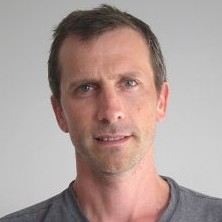
\includegraphics[height=.2\linewidth]{Pictures/FrancisV2.jpeg}}
        \end{minipage}}\\
	& & \\[.1cm]
	$\diamond$ & \multirow{2}{.82\linewidth}{Drori, T (2020). ``Efficient first-order methods for convex minimization: a constructive approach.'' Mathematical Programming 184(1).} & {\begin{minipage}{0.18\linewidth}{
\includegraphics[height=.2\linewidth]{Pictures/Yoel.jpg}}\end{minipage}}\\
	& & \\[.1cm]
$\diamond$ & \multirow{2}{.82\linewidth}{Drori, T (2022). ``On the oracle complexity of smooth strongly convex minimization.'' Journal of Complexity 68.} & {\begin{minipage}{0.18\linewidth}{
\includegraphics[height=.2\linewidth]{Pictures/Yoel.jpg}}\end{minipage}}\\
	& & \\[.1cm]
$\diamond$ & \multirow{2}{.82\linewidth}{Barr\'e, T, Bach (2023). ``Principled analyses and design of first-order methods with inexact proximal operators.'' Mathematical Programming 201(1).} & {\begin{minipage}{0.18\linewidth}{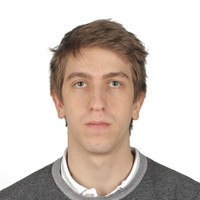
\includegraphics[height=.2\linewidth]{Pictures/mathieu.jpeg}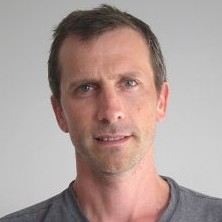
\includegraphics[height=.2\linewidth]{Pictures/FrancisV2.jpeg}}
        \end{minipage}}\\
	& & \\[.1cm]
$\diamond$ & \multirow{2}{.82\linewidth}{T, Drori (2023). ``An optimal gradient method for smooth strongly convex minimization.'' Mathematical Programming 199(1).} & {\begin{minipage}{0.18\linewidth}{
\includegraphics[height=.2\linewidth]{Pictures/Yoel.jpg}}\end{minipage}}\\
	& & \\[.1cm]
$\diamond$ & \multirow{2}{.82\linewidth}{Weibel, Gaillard, Koolen, T (2025). ``Optimised projection-free algorithms for online learning: construction and worst-case analysis.''} & {\begin{minipage}{0.18\linewidth}{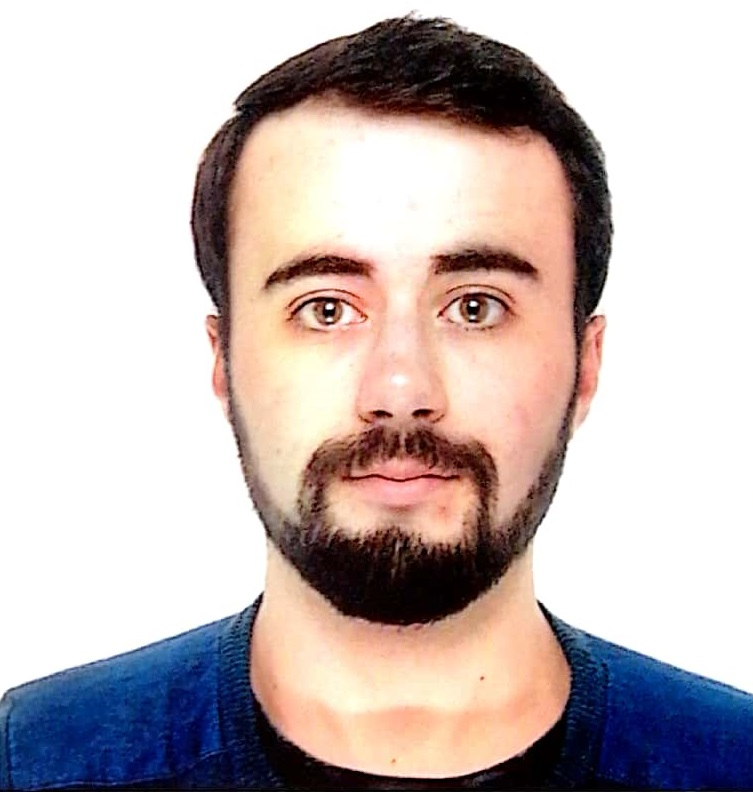
\includegraphics[height=.2\linewidth]{Pictures/julien_weibel.jpg}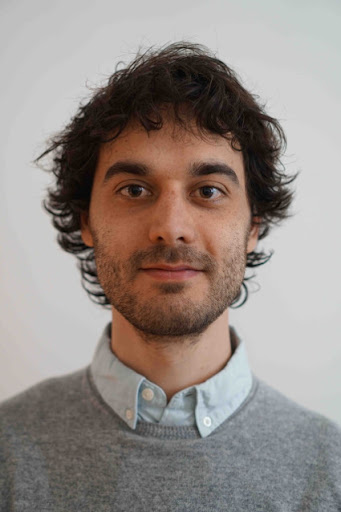
\includegraphics[height=.2\linewidth]{Pictures/Pierre.jpg}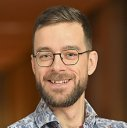
\includegraphics[height=.2\linewidth]{Pictures/wouter.jpeg}}
        \end{minipage}}\\
	& & \\[.1cm]
\end{tabular}

\end{frame}



\begin{frame}
	\Large
	\tableofcontents
\end{frame}
\section{Design techniques}
\subsection{Design via idealized algorithms}
\begin{frame}
	\Large
	\tableofcontents [currentsection, hideothersubsections]
\end{frame}

\begin{frame}{SSEP}

\end{frame}


\begin{frame}
	\Large
	\tableofcontents
\end{frame}
\subsection{Design via convex relaxations}
\begin{frame}
	\Large
	\tableofcontents [currentsection, hideothersubsections]
\end{frame}
\begin{frame}{Relax}

\end{frame}


\begin{frame}
	\Large
	\tableofcontents
\end{frame}
\subsection{Design via brutal approaches}
\begin{frame}
	\Large
	\tableofcontents [currentsection, hideothersubsections]
\end{frame}

\begin{frame}{Nonlinear SDPs}

\end{frame}




\begin{frame}
	\Large
	\tableofcontents
\end{frame}
\section{Concluding remarks}
\begin{frame}
	\Large
	\tableofcontents [currentsection, hideothersubsections]
\end{frame}
\begin{frame}{...what did we learn?}

\end{frame}




\end{document}


















